\chapter{Robust feasibility checking}\label{chap:appendixA}

% \begin{figure} [t]
%     \centering
%     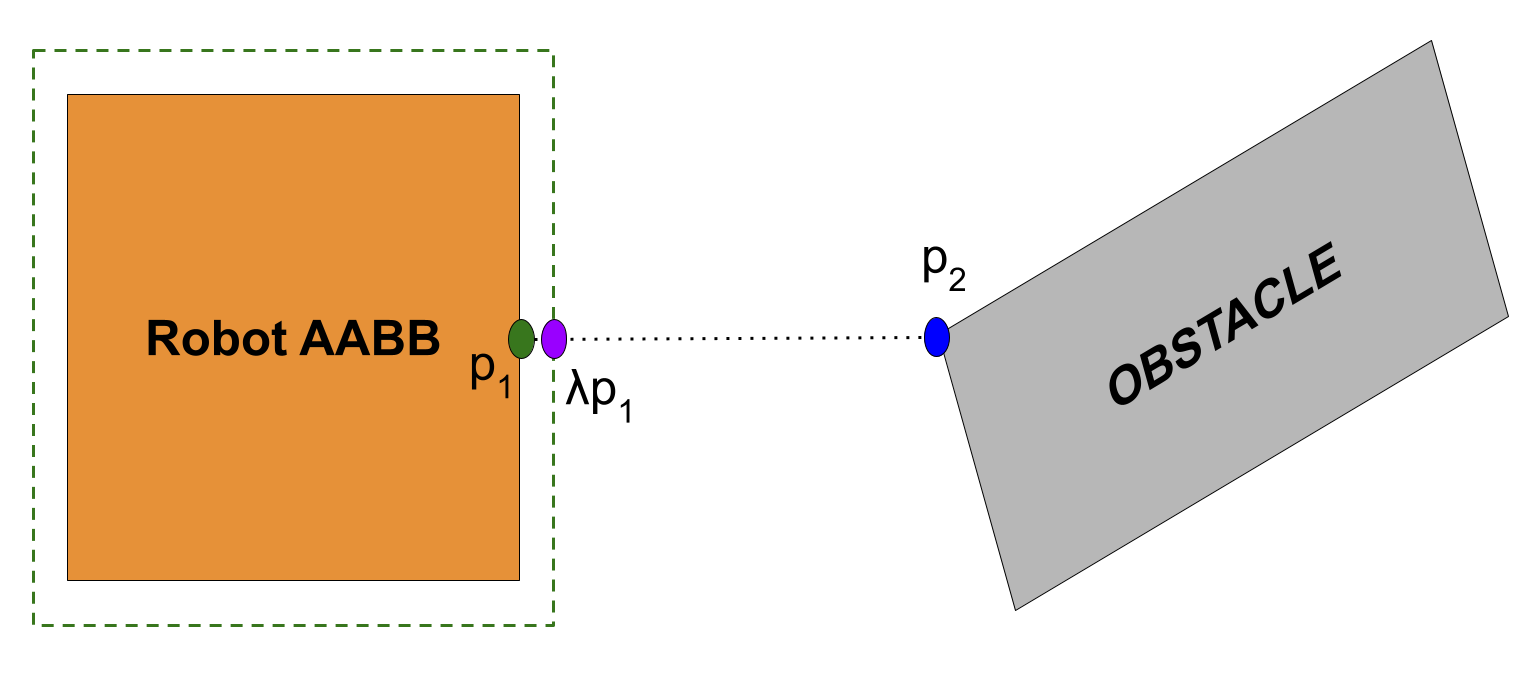
\includegraphics[width=0.8\linewidth]{figures/appendix/CCellipse.png}
%     \caption{Collision checking given a uniform scaling of the robot AABB.}
%     \label{fig:appendix_A}
% \end{figure}

% Given a current robot AABB, this proof aims to show that the closest point on the robot to an obstacle remains the closest point after uniform scaling, and that the closest point of the obstacle to the robot also remains unchanged (see Figure~\ref{fig:appendix_A}).

% Let $A$ and $B$ be two convex sets. 
% This assumption holds for the collision test presented in Section~\ref{sec:robust_CC} as the robot AABB is a convex shape, and the environment is decomposed into convex shapes.
% Let \( p_1 \in A \) such that \( p_1 = \arg \min_{a \in A} \|a - b\| \, \forall b \in B \), and \( p_2 \in B \) such that \( p_2 = \arg \min_{b \in B} \|a - b\| \, \forall a \in A \).
% Also let $\lambda A, \lambda \geq 1$ be a uniform scaling of $A$.

% One want to show that:
% \begin{enumerate}
%     \item The projection of $p_1$ due to the scaling remains the closest point to the obstacle.
%     \item $p_2$ remains the closest point to the projection of $p_1$. 
% \end{enumerate}
% \[
%     \left\{
%     \begin{aligned}
%         \lambda p_1 &= \argmin_{a \in A} \|\lambda a - b\| \, \forall b \in B \\
%         p_2 &= \argmin_{b \in B} \|\lambda p_1 - b\|
%     \end{aligned}
%     \right.
% \]

% \paragraph{1.}
% Let \( a \in A \) and \( b \in B \).
% One can express the following relationship:
% \[
% \|\lambda a - b\| = \lambda \left\|a - \frac{b}{\lambda}\right\|,
% \]
% where \(\frac{b}{\lambda} \in B\) because \(B\) is convex. 
% Therefore, one gets:
% \[
% \arg \min_{a \in A} \left\|a - \frac{b}{\lambda}\right\| = \arg \min_{a \in A} \|a - b\| = p_1,
% \]
% which implies:
% \[
% \arg \min_{a \in A} \|\lambda a - b\| = \lambda p_1.
% \]

% \paragraph{2.}
% Let \( b \in B \), \( b \neq p_2 \) such that:

% \[
% \|\lambda p_1 - b\|^2 = \|\lambda p_1 - p_2\|^2 + \|p_2 - b\|^2,
% \]
% and since \( p_2 \neq b \), one gets \( \|p_2 - b\|^2 > 0 \). 
% Therefore, \( \|\lambda p_1 - b\| > \|\lambda p_1 - p_2\| \), which implies \( \arg \min_{b \in B} \|\lambda p_1 - b\| = p_2 \).

Sampling-based algorithms generate global trajectories by combining multiple continuous local trajectories.
During the process, each of these local trajectories are subject to collision checks to determine their feasibility.
However, in this thesis, the collision check is extended to include a more general feasibility test, which also accounts for the control input space. 
This extension ensures that the generated trajectories are not only free from obstacles but also prevent control inputs from reaching saturation. 
Additionally, it accounts for uncertainty in both the state and control input spaces, further enhancing the robustness of the trajectories.
The following appendix describes how these extended feasibility check is performed to ensure the robustness of each local trajectory in this context.
It is important to note that these test is not continuous; rather, it is performed along a discrete representation of the local trajectories.

\paragraph{Robust collision checking}

In this thesis, collision detection is performed using the widely used C implementation of PyBullet~\cite{cBullet}, which operates as follows: 
\begin{enumerate}
    \item It starts with a broad-phase collision detection using \myglsentry{AABBs} to quickly eliminate pairs of objects that are too far apart to collide, allowing the more computationally intensive collision checks to focus only on pairs that are potentially close to each other.
    \item Then, it performs a narrow-phase collision detection that, after potential collision pairs are identified, checks for each pair. 
    For each identified potential collision pair, this phase uses a more precise robot representation (as defined by the user) and specialized collision algorithms to detect actual intersections and determine contact points, normals, and penetration depths.
\end{enumerate}

Extending this procedure to account for robot state uncertainty aims to verify that the resulting extended bounding volume, which the robot may occupy due to the uncertainty, is clear of obstacles.
In this work, such bounding volume is computed by considering only the uncertainty in the position subspace for simplicity (i.e., the $\{x,y,z\}$-subspace for the quadrotor or the $\{x,y\}$-subspace for the differential drive robot).

This work employ a robust collision check generic to all free flying robots that operates as followed:
\begin{enumerate}
    \item As mentioned above, the first phase performs a broad collision detection considering the current robot AABB. 
    Therefore, in the robust collision detection of this work, this phase involves creating an extended AABB by scaling the current robot AABB in all directions according to their respective uncertainty radii as shown in Figure~\ref{fig:CCmethods}. 
    \item The narrow phase approach leverage a fine robot representation.
    However, generating the accurate extended collision mesh that incorporates uncertainty, required for the second phase, is challenging, as it involves deforming all the vertices of the robot mesh.
    To address this, this work approximate the extended collision mesh by sampling on the surface of the uncertainty ellipsoid bounding box defined by the uncertainty tube radii (see Figure~\ref{fig:CCmethods}). 
    While this method accurately approximates the true extended collision shape, it requires multiple calls to the collision-checking function for each robot state tested.
\end{enumerate}

\begin{figure}[htp]
    \centering
    % Row 1
    \begin{subfigure}{0.4\textwidth}
        \centering
        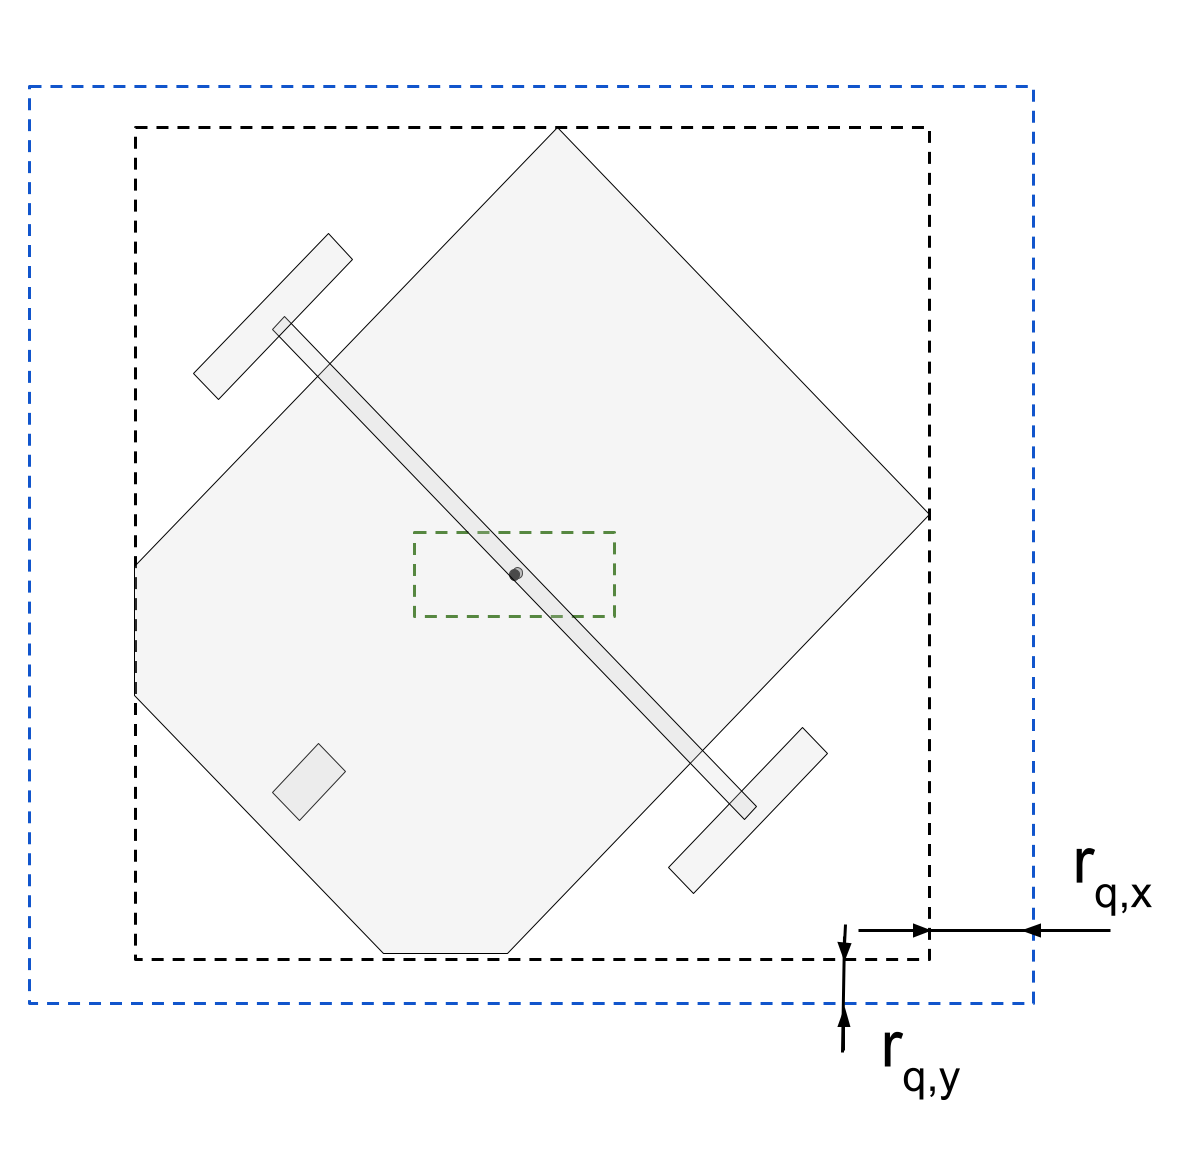
\includegraphics[width=\linewidth]{figures/samp/CC2.png}
        \caption{}
        \label{fig:CC1}
    \end{subfigure}
    % \hfill
    \begin{subfigure}{0.4\textwidth}
        \centering
        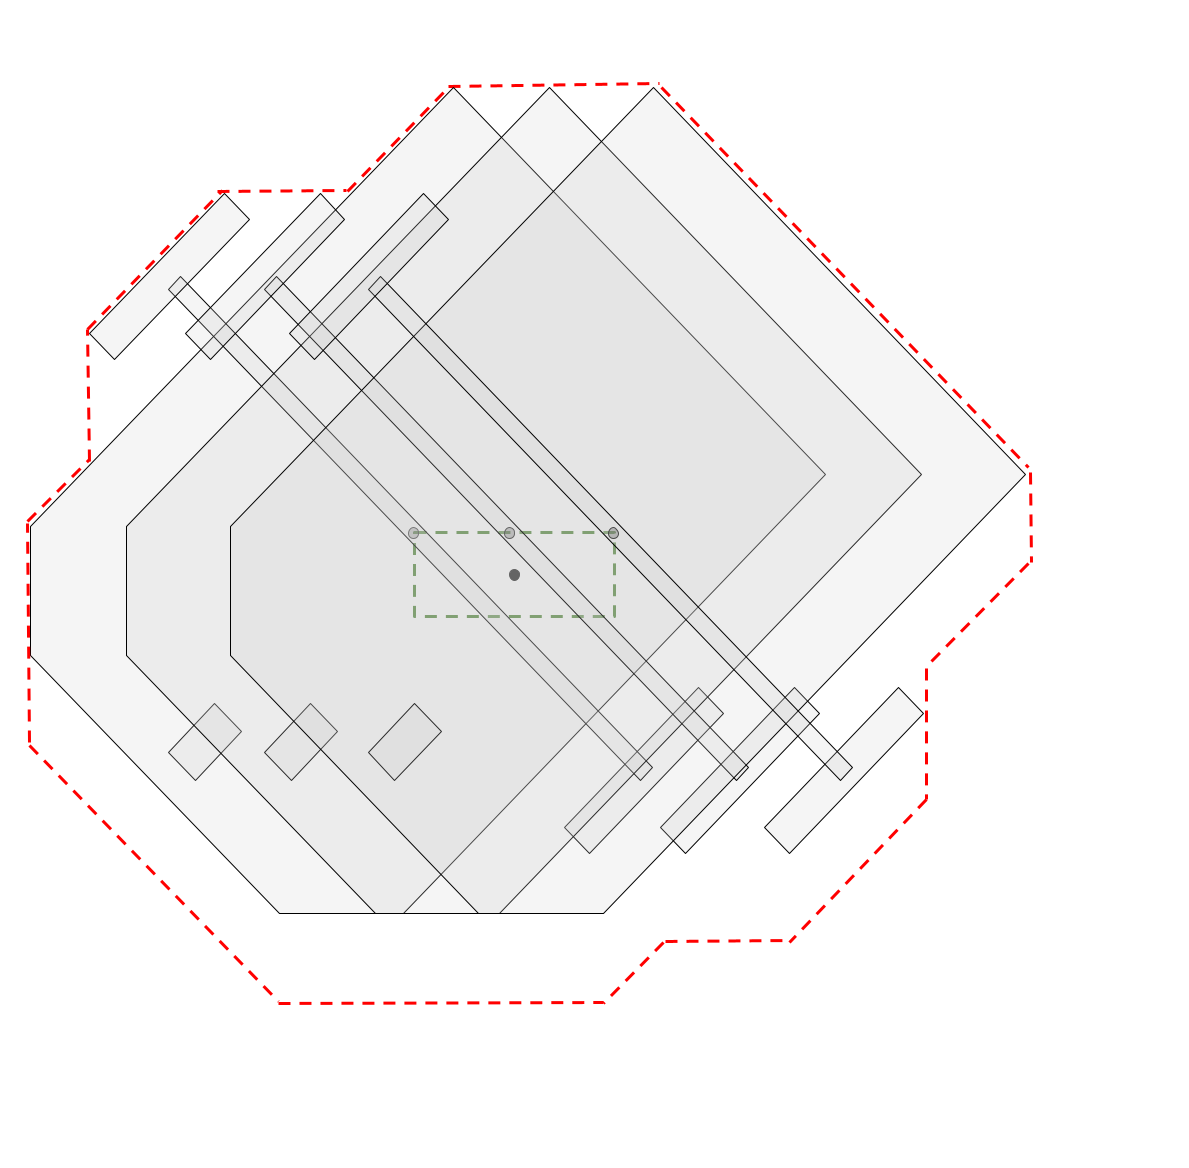
\includegraphics[width=\linewidth]{figures/samp/CC3.png}
        \caption{}
        \label{fig:CC2}
    \end{subfigure}
    
    % Row 2
    \begin{subfigure}{0.4\textwidth}
        \centering
        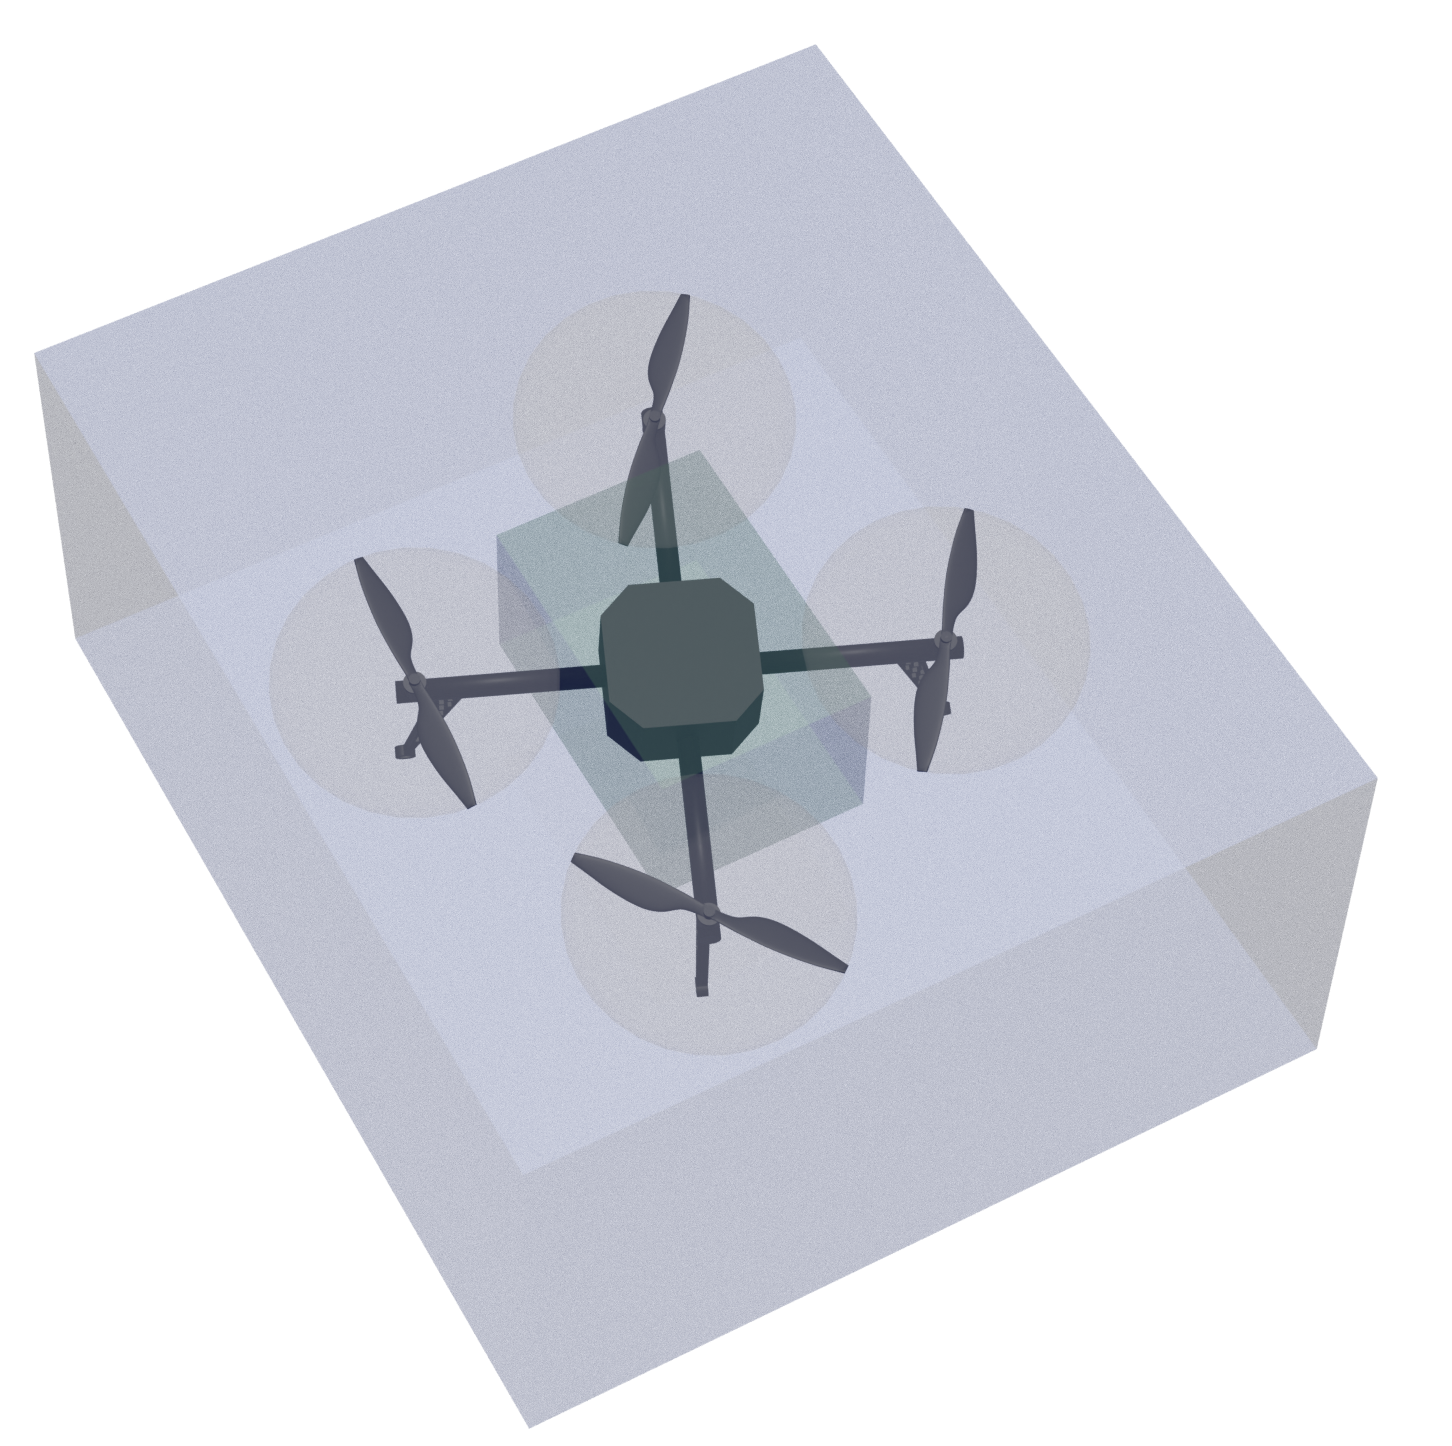
\includegraphics[width=\linewidth]{figures/appendix/CCdrone1.png}
        \caption{}
        \vspace{-0.3cm}
        \label{fig:CC3}
    \end{subfigure}
    % \hfill
    \begin{subfigure}{0.4\textwidth}
        \centering
        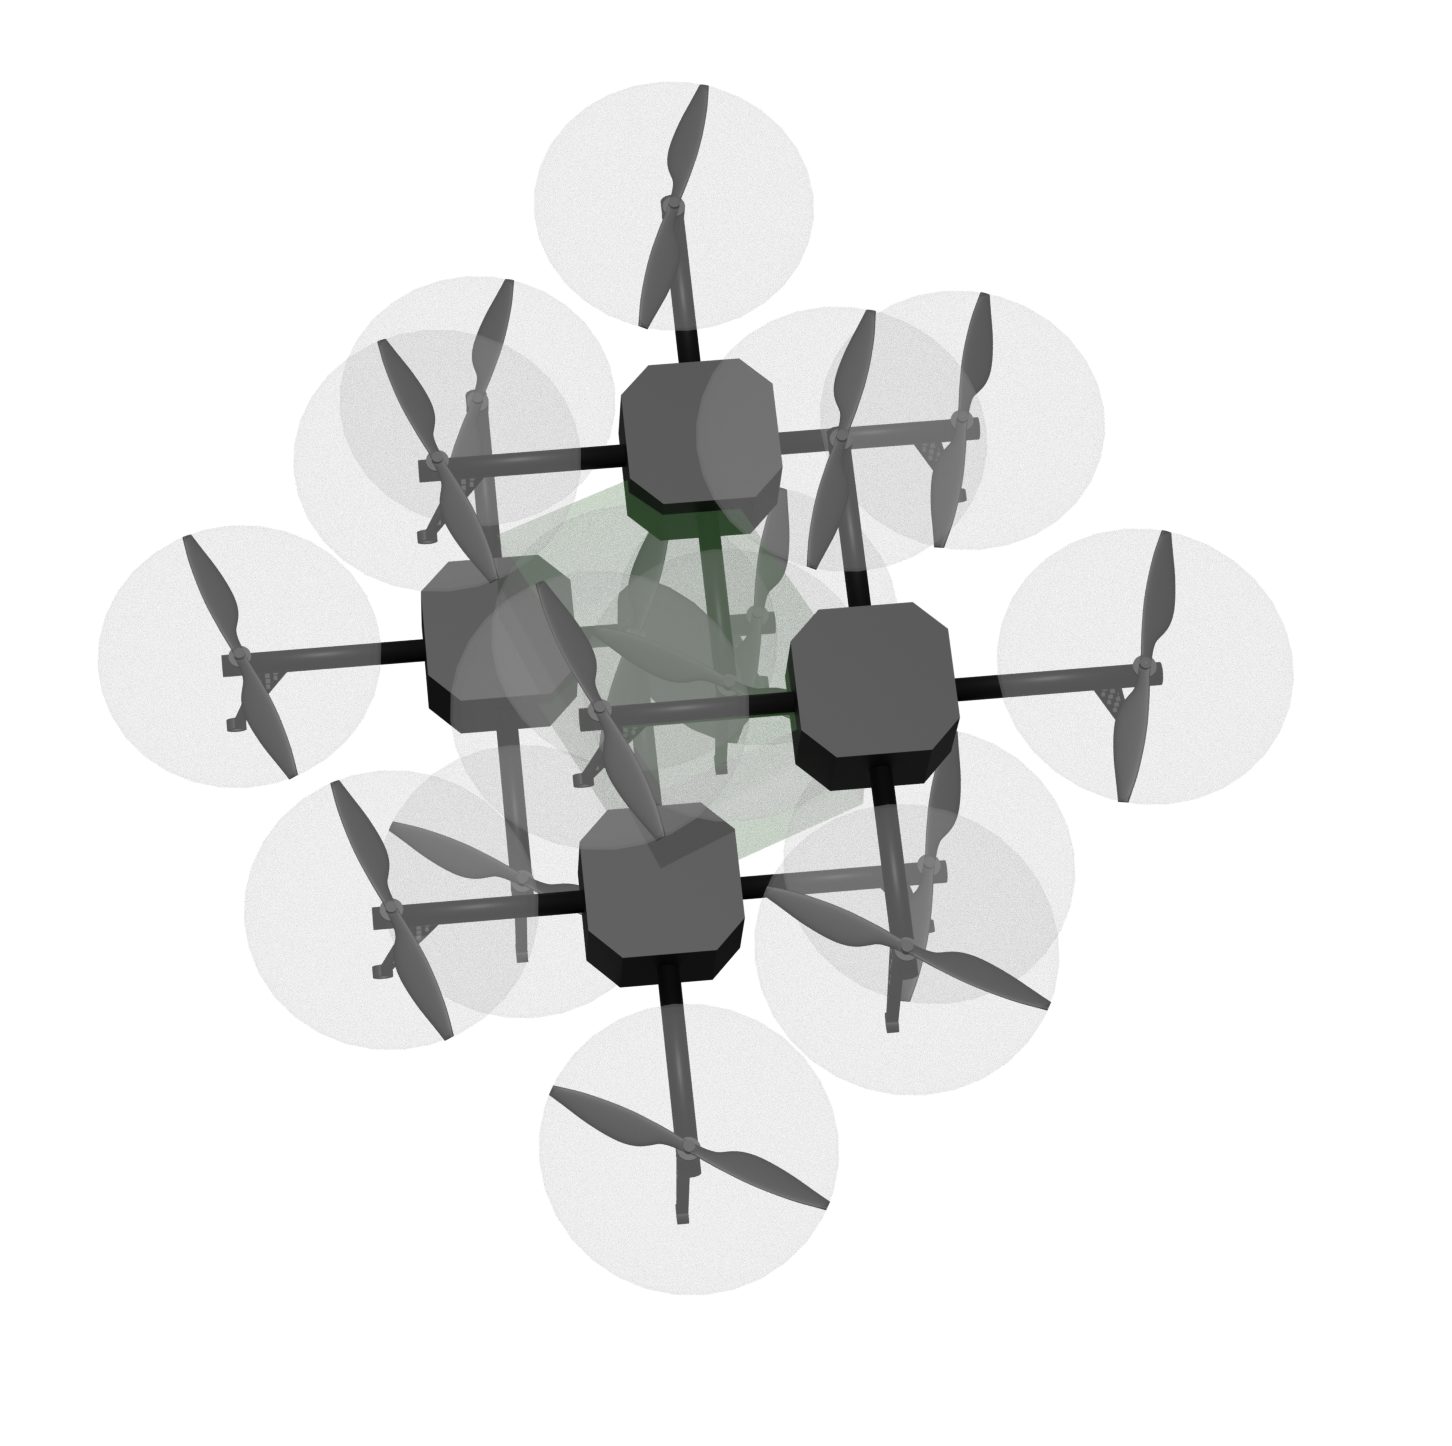
\includegraphics[width=\linewidth]{figures/appendix/CCdrone2.png}
        \caption{}
        \vspace{-0.3cm}
        \label{fig:CCall}
    \end{subfigure}

    \caption{Figure showing the resulting shapes tested for collisions: (a) differential drive robot extended AABB, 
    (b) sampling-based approximated uncertain mesh, for a differential drive robot with its associated uncertainty ellipsoid bounding box (green), (c) quadrotor extended AABB, and (d)
    sampling-based approximated uncertain mesh, for a quadrotor with its associated uncertainty ellipsoid bounding box (green).
    Note that not all the sampled configurations are displayed for clarity.}
    \label{fig:CCmethods}
\end{figure}

Although the methods employed in this thesis for robust collision checking rely on the uncertainty ellipsoid bounding box computed using Equation~\ref{eq:radius}, the tubes are represented by ellipsoids in the various figures of this manuscript for smoother visualization.

\paragraph{Robust saturation checking}
Then, in this manuscript, the feasibility check is not restricted to the aforementioned collision test, but it also verifies that the robot control inputs does not saturate.
This test is performed by checking that the tube associated with each control input remains in its feasibility domain.
An example of infeasible input for the quadrotor case is presented in Figure~\ref{fig:invalid_inputs}, where the tube (green) around the nominal control input of the first actuator (blue) exceeds the maximum allowed input (red).
Note that this simple test is less costly than the robust collision checking one, it is therefore performed first by mean of computational efficiency. 

\begin{figure} [htp]
    \centering
    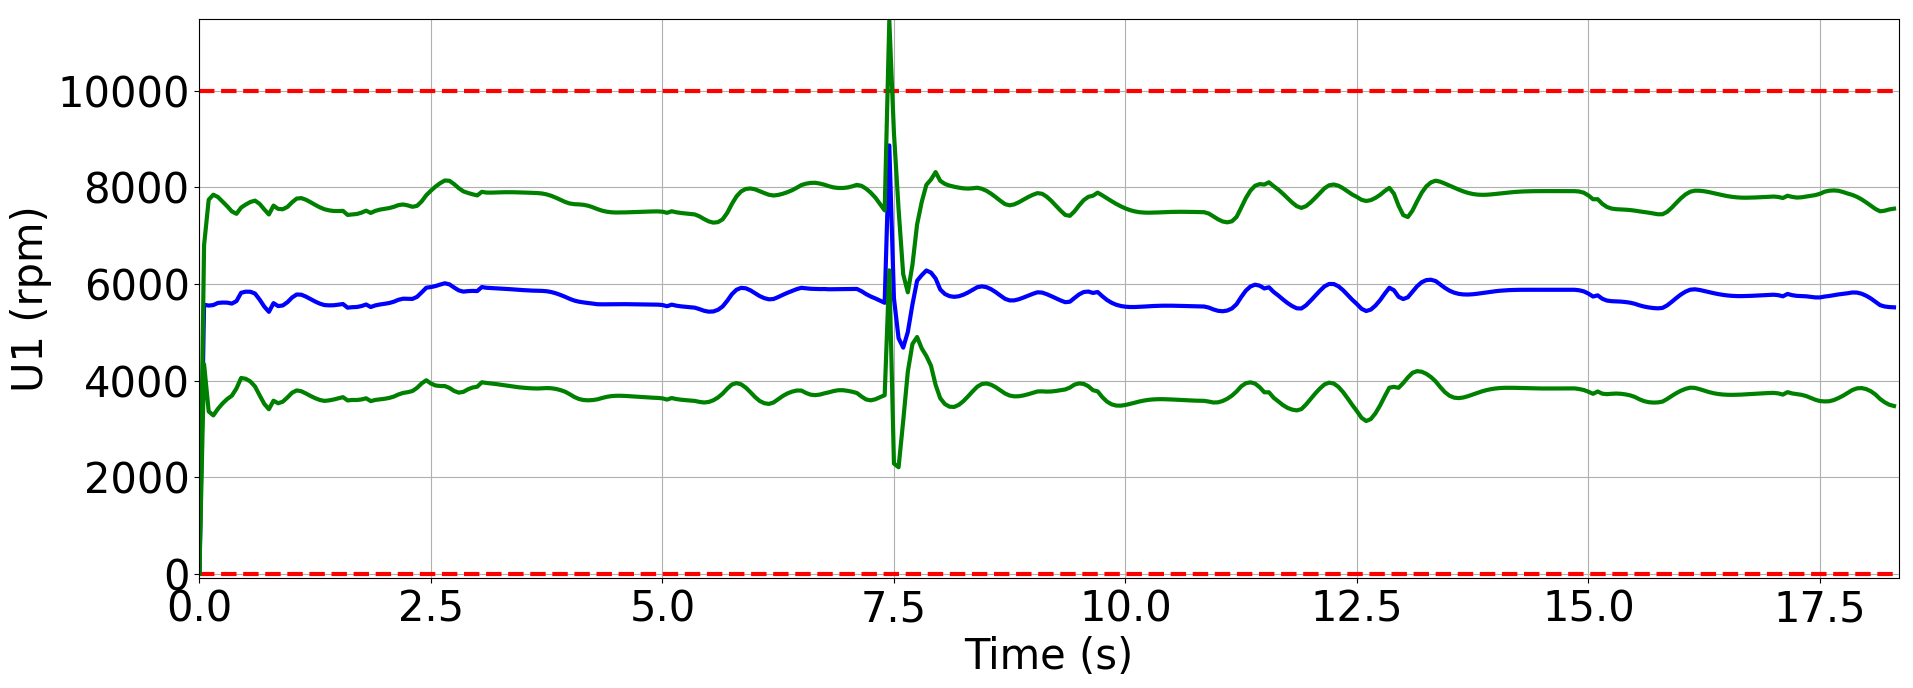
\includegraphics[width=0.8\linewidth]{figures/samp/Invalid_Inputs.png} 
    \caption{Non-robust nominal control input profile for the first rotor of a quadrotor (blue) along a specified trajectory, depicted with its uncertainty tube (green) and the control input limits (red).}%
    \label{fig:invalid_inputs}%
\end{figure}